\vspace{-.15in}\section{Research Plan and Methodology}
\label{sec:rep}\vspace{-.075in}

\xxx strengthens the reliability of datacenter 
computing with a holistic methodology. This section first proposes \falcon 
(\S\ref{sec:protocol}), a fast consensus protocol, it then leverages \falcon to 
build a scheduler (\S\ref{sec:scheduler}) and a VM replication infrastructure 
(\S\ref{sec:vm}) to improve the availability of applications ran by these 
infrastructures. Finally, this section describes research plan 
(\S\ref{sec:plan}).
% The first two objectives include preliminary results. 

\vspace{-.15in}\subsection{Objective 1: Building Fast Distributed Consensus via
RDMA}\label{sec:protocol}\vspace{-.075in}

This section describes a performance problem (\S\ref{sec:latency-problem}) in 
existing \paxos protocols and presents \falcon (\S\ref{sec:falcon}), a 
fast \paxos protocol by leveraging RDMA.

\vspace{-.15in}
\subsubsection{Problem: consensus latency of existing \paxos 
protocols are slow and unscalable} 
\label{sec:latency-problem}\vspace{-.075in}

% P1: as mentioned in background, a key reason is thread interleavings, 
% so we need to reason about the general patterns we have. Or we say our 
% methodology is just like pattern matching.
% Traditional \paxos protocols incur high consensus latency because they go 
% through OS kernels and software TCP/IP layers. In this 
% section, \S\ref{sec:problem} analyzes this latency problem and its poor 
% scalability in detail, and then presents our new RDMA-based \paxos 
% protocol called \falcon (\S\ref{sec:falcon}).

% First, mainly introduce the problems in traditional protocols.
% Due to the strong fault-tolerance of \paxos, it is widely served in many 
% systems. For instance, Scatter~\cite{scatter:sosp11} runs 8$\sim$12 replicas in 
% each \paxos group to order client requests, and it lets replicas respond 
% requests in parallel. A bigger group size will improve Scatter throughput. 
% Moreover, recent state machine replication (SMR) 
% systems~\cite{eve:osdi12,rex:eurosys14,crane:sosp15} use \paxos to greatly 
% improve the availability of
% general server programs.

Despite the wide deployments of \paxos (\S\ref{sec:consensus}), its high 
consensus latency makes many software applications suffer. For efficiency, 
\paxos typically assigns one replica as the leader to propose consensus 
requests, and the other replicas as backups to agree on requests. To 
agree on an input, at least one message round-trip is required between the 
leader and a backup. A round-trip causes big latency (hundreds of \us) as it 
goes through various software layers (\eg, OS kernels).

% This 
% latency may be acceptable for leader election~\cite{chubby:osdi,zookeeper} or 
% heavyweight transactions~\cite{crane:sosp15,eve:osdi12}, but undesirable for
% key-value store applications~\cite{redis,memcached}.

As replica group size increases, \paxos consensus latency scales poorly: it increases
drastically~\cite{scatter:sosp11} due to the linearly increasing number of 
consensus messages. One common approach to improve \paxos scalability is 
leveraging parallel techniques such as multithreading~\cite{zookeeper, 
spaxos:srds12} or asynchronous IO~\cite{crane:sosp15, libpaxos}. However, the 
high TCP/IP round-trip latency still exists, and synchronizations in these 
techniques frequently invoke expensive OS events such as context switches.

Our preliminary study (Figure~\ref{fig:scalability}) ran four \paxos-like 
protocols~\cite{zookeeper, spaxos:srds12, crane:sosp15, libpaxos} on 40Gbps 
network with only one client sending consensus requests. When changing the 
replica group size from 3 to 9, the consensus latency of three protocols 
increased by \tradlatencyincreaselow to \tradlatencyincreasehigh, and 
\systemcostlow to \systemcosthigh of this increase was in OS kernel. The only
exception is S\-Paxos~\cite{spaxos:srds12} because it batches requests from backups
and invokes consensus when the batch is full. More replicas causes shorter time
to form a batch, but bacthing causes its consensus latency the highest with
less replicas.

% Second, briefly mention the problem in DARE. and its scalability bottleneck.
RDMA appears a promising approach (\S\ref{sec:consensus}) to speed up \paxos. 
However, fully exploiting RDMA speed in software systems is widely considered 
challenging by the community~\cite{pilaf:usenix14,herd:sigcomm14,
farm:sosp15,dare:hpdc15}. For instance, \dare~\cite{dare:hpdc15} presents a
two-round, RDMA-based \paxos protocol in a sole-leader manner: leader does all 
RDMA workloads and backups do nothing. Although \dare was fast with 3$\sim$5 
replicas, our study (Figure~\ref{fig:scalability}) shows that \dare's sole-leader
nature incurred a scalability bottleneck and thus a linearly increasing consensus latency.

\vspace{-.15in}\subsubsection{Falcon: a fast, scalable RDMA-based \paxos 
protocol} 
\label{sec:falcon}\vspace{-.075in}

Our key observation is that we should carefully separate RDMA workloads among
the leader and backups, especially in a scalability-sensitive context. 
Intuitively, we can let both leader and backups do RDMA writes directly on 
destination replicas' memory, and let all replicas poll their local memory to 
receive messages.

Although doing so will consume more CPU resources than a sole-leader 
protocol~\cite{dare:hpdc15}, it has two major benefits. First, both leader and 
backups participate in consensus, making it possible to reach consensus 
with only one round~\cite{paxos:practical}. Second, all replicas can just 
receive consensus messages on their bare, local memory. An analogy is threads 
receiving other threads' data via bare memory, a fast and scalable computation 
pattern.

We propose \falcon,\footnote{We name our protocol after
falcon, one of the fastest birds.} a new RDMA-based \paxos protocol and its
runtime system. In \xxx, all replicas directly write to destination
replicas' memory and poll messages from local memory to receive messages, and 
our runtime system handles other technical challenges such as checking message 
delivery and recovering replica failures.

\begin{figure}[h]
    \centering
    \begin{minipage}{.48\textwidth}    
        \vspace{-.18in}
        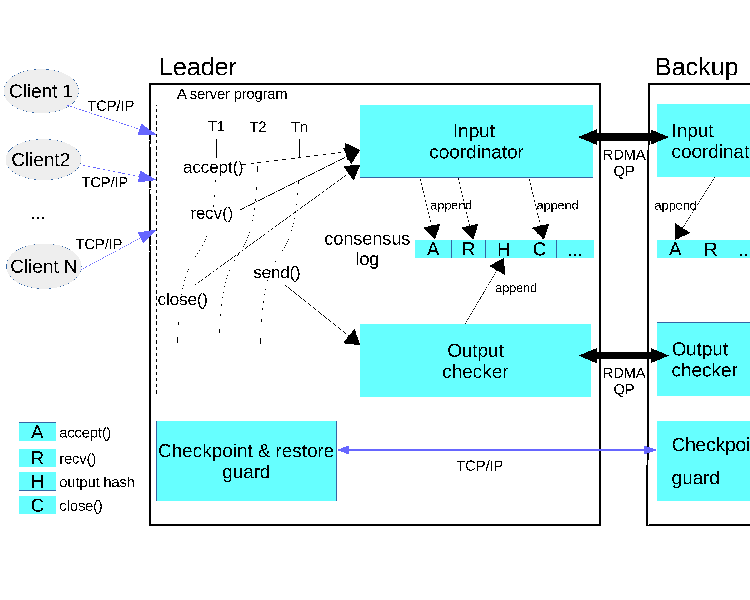
\includegraphics[width=0.31\textheight]{figures/arch.ps}
        \vspace{-.35in}         
        \caption{The \falcon protocol architecture. Protocol components are 
shaded (and in blue color).}
        \label{fig:falcon-arch}
    \end{minipage}
    \centering
    \begin{minipage}{0.48\textwidth}
        \vspace{-.25in}
        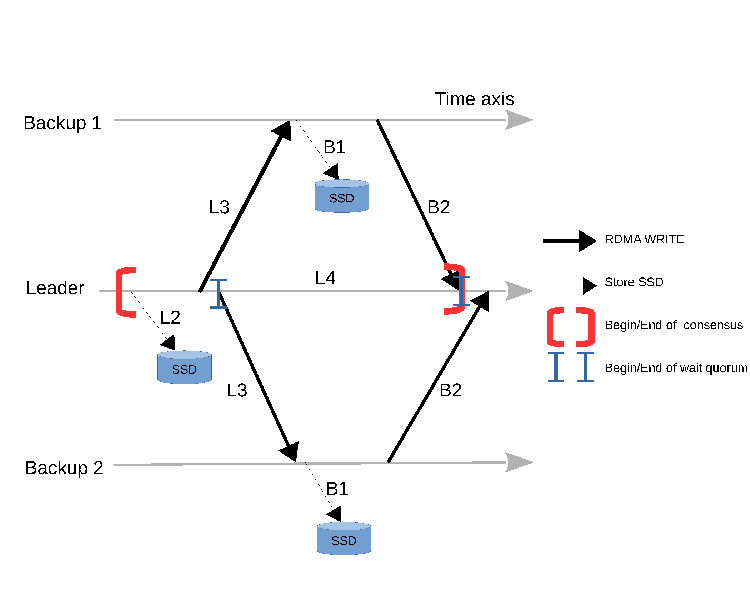
\includegraphics[width=0.34\textheight]{figures/consensus.ps}
        \vspace{-.32in}
        \caption{RDMA-powered consensus algorithm.}
        \label{fig:falcon-protocol}
    \end{minipage}
\end{figure}



\falcon supports unmodified applications. \falcon automatically deploys the 
same application on multiple replicas, intercepts the application's 
network inputs from its inbound socket calls (\eg, \recv) with a Linux 
technique called LD\_PRELOAD, and invokes its RDMA-based consensus protocol to 
enforce same network inputs across replicas. Figure~\ref{fig:falcon-arch} 
shows \falcon's architecture on the leader replica with three key components: 
an input consensus coordinator, an in-memory consensus log, and a guard that 
checkpoints and recovers application execution states.

Figure~\ref{fig:falcon-protocol} shows \falcon's consensus algorithm in normal 
case. The leader first executes the actual inbound socket call to get and store 
the actual inputs, it then invokes consensus across replicas. All 
solid arrows (\textbf{L3} and \textbf{B2}) are direct RDMA writes to remote 
replicas' memory. All replicas poll from their own bare memory to receive 
consensus messages. To handle replica failures, all replicas persistently log 
inputs to local SSD storage (\textbf{L2} and \textbf{B1}). For these writes, 
the sending replicas only need to copy the data to local RDMA NIC and then the 
writes finish, \falcon is scalable when more backup replicas are added.

% Three figures. First, falcon arch. Second, consensus protocol. Third, falcon 
% results compared to traditional ones and DARE.



\begin{wrapfigure}{r}{7cm}
  \vspace{-.1in}
  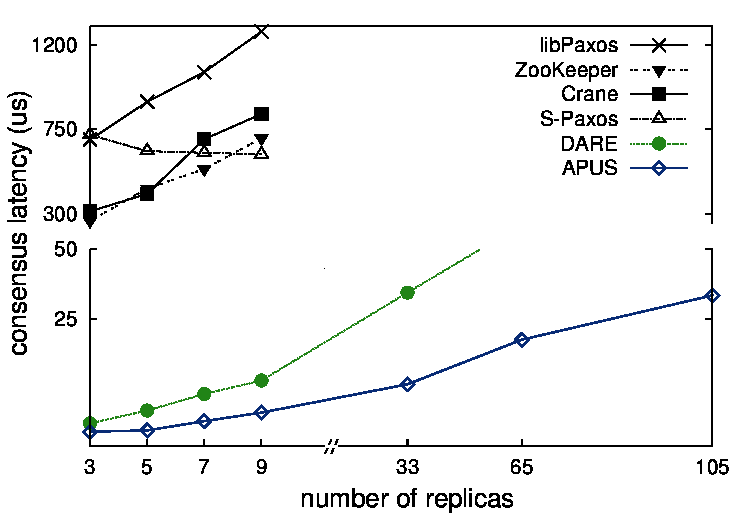
\includegraphics[width=7cm]{figures/traditional_paxos_latency.ps}\\
  \vspace{-.3in}
  \caption{Consensus latency of six \paxos protocols. Both X and Y axes are 
broken to fit in all these protocols. \falcon achieves the smallest consensus 
latency.}
  \label{fig:scalability}
\end{wrapfigure}

% \begin{figure}[!htb]
% \centering
% 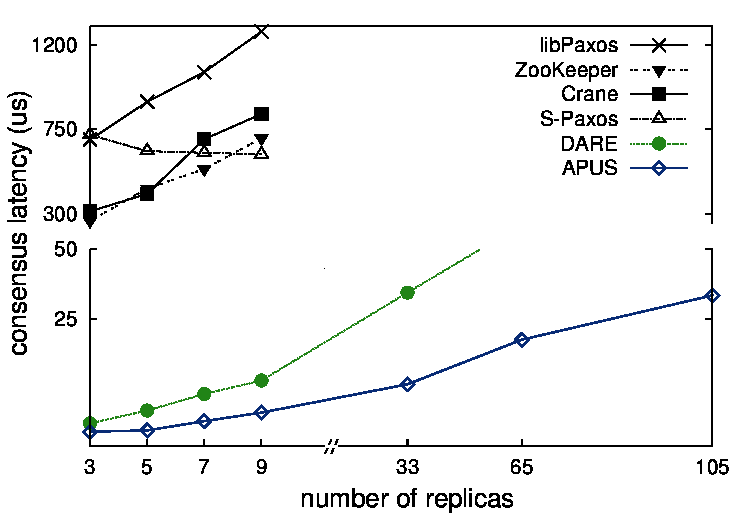
\includegraphics[width=0.25\textheight]{figures/traditional_paxos_latency.ps}
%         \vspace{-.2in}
%         \caption{Consensus latency of six \paxos protocols. \falcon is fastest 
% and scales the best.}
%         \label{fig:scalability}
% \end{figure}

\para{Preliminary results.} We implemented a \falcon prototype with two steps. First,
to support unmodified applications, we implemented its socket-intercepting protocol,
published in SOSP 2015~\cite{crane:sosp15}. \falcon was able to support five widely
used server applications (\eg, \mysql) without modifying them. Second, we implemented its
RDMA-powered consensus algorithm on a 40bps RDMA network. Figure~\ref{fig:scalability}
shows \falcon performance with 5 existing consensus protocols. To analyze the scalability
of our algorithm, we ran \falcon and \dare on up to 105 replicas. \falcon's consensus latency 
outperforms 4 popular \paxos  protocols by \comptradlow to \comptradhigh on 3 to 9 replicas.
\falcon is  faster than \dare by up to \fasterDARE.
% When changing the replica group size 
% from 3 to 105 (a 35x increase), \falcon's consensus latency increases merely 
% from \xxxlatencythree \us to \xxxlatencyonezerofive \us (a \xxxscalability, 
% sub-linear increase).
% Crane. Falcon. Say Crane is first version. Falcon 
% totally subsumes Crane. Falcon also has initial results.



\para{Future work.} Since \falcon is the keystone of our objectives, this 
proposal plans to further improve its practicality in two directions: 
(1) evaluate its performance and generality on more latency-critical applications, 
and (2) study its protocol robustness on failure scenarios, including leader
election and adding/removing replicas.

\vspace{-.15in}\subsection{Objective 2: 
building a fault-tolerant scheduler to improve 
application availability}\label{sec:scheduler}\vspace{-.075in}

Many existing schedulers have adopted \paxos to improve availability for 
themselves. Typically, they use \paxos to replicate their essential components 
such as a controller, which handles scheduling computation jobs to run on 
resources. In normal case, only one leading controller does the real 
work, and the others standby to cope with the leader's failure. Unfortunately, 
most applications running by these schedulers have not been made 
highly-available (although minor applications implement a replication 
approach~\cite{mapreduce,dolly:nsdi13}).

A naive approach to achieve high application availability could be implementing 
a \paxos within each application. However, this approach has two major issues. 
First, \paxos is notoriously difficult to 
understand~\cite{raft:usenix14,paxos:simple}, implement~\cite{paxos:practical, 
paxos:live}, or test~\cite{modist:nsdi09,demeter:sosp11}, thus developing a 
\paxos protocol for each application is widely considered a 
nightmare~\cite{modist:nsdi09,demeter:sosp11,paxos:live} for application 
developers.

The second issue is, the scheduler may defeat \paxos due to unawareness of the 
application's \paxos replication logic. For instance, if an application submits 
multiple copies of the same computation job to the scheduler, the scheduler may 
incorrectly schedule several copies on the same computer (it should schedule 
each copy on different computers to achieve \paxos fault-tolerance).

\vspace{-.15in}\subsubsection{\tripod: a first fault-tolerant scheduler 
architecture} 
\label{sec:scheduler-arch}\vspace{-.075in}

% ,\footnote{We name our system after 
% the ancient Chinese three-legged tripod, a reliable, multi-purpose container.}
This section proposes the design of \tripod, a scheduler infrastructure that 
automatically provides high-availability to general applications. \tripod 
is integrated with a widely used scheduler \mesos~\cite{mesos:nsdi11} and 
\falcon (\textbf{Objective 1}). To avoid the two aforementioned issues 
(\S\ref{sec:scheduler}), \tripod chooses 
to integrate \paxos in a scheduler, not in applications. To achieve high
application availability, unlike existing schedulers which let only one 
controller schedule jobs, \tripod runs replicas of the same job using replicas 
of controllers: after controllers agree on a new job with \falcon, \tripod lets 
each controller independently schedule an copy of this job.

% Doing so has three benefits. First, \tripod's \paxos acts as a single, general 
% fault-tolerance service to applications. We can just leverage existing 
% verification tools~\cite{modist:nsdi09,demeter:sosp11} to make sure that our 
% \falcon protocol is robust and correct, and then we can benefit many 
% applications. Second, application developers can now just focus on their own 
% application logic, greatly saving development time and money. Third, now 
% \tripod's own scheduler can handle the replication logic and do careful, 
% replication-aware scheduling for jobs  (\S\ref{sec:workflow}). 


% To 
% ahieve application fault-tolerance, 



% In an implementation level, \tripod integrates \mesos~\cite{mesos:nsdi11}, a 
% widely used cluster management system, with a new RDMA-enabled \paxos 
% protocol~\cite{falcon:github}. Compared to a prior RDMA-enabled \paxos 
% protocol~\cite{dare:hpdc15}, our new protocol can support general programs 
% transparently without modifications.

Figure~\ref{fig:scheduler-arch} depicts \tripod's architecture, and its key 
components are shaded (and in blue). To illustrate how \tripod works in an 
application perspective, this figure shows two applications, Hadoop and MPI. 
Each application has a \emph{replica strength} (\vv{R}) to denote the level of 
fault-tolerance it demands. This value is either 1 or equals the number of 
replicas of controllers in \tripod.

By default, each application has \vv{R=1}, which means that this application 
does not need replication. For such a default setting, \tripod runs the job as 
is without replication, like a typical cluster management system (\eg, Mesos).

In this figure, Hadoop's \vv{R} is 3, which means that it wants to replicate 
each of its job with three copies for high-availability. Suppose Hadoop 
submits two jobs to the leader controller, each has different shapes (triangle 
or hexagon). The leader controller then invokes a consensus on each job across 
controllers. Once a consensus is reached, each controller assigns the same job 
on different slave machines. The leader controller directly returns its 
computation result to the Hadoop scheduler. Standby controllers ignore the 
results unless the same mechanism is triggered.
%  unless a tail-tolerance mechanism is triggered 
% (\S\ref{sec:workflow})

% Hack: use eps to avoid the 1MB terrible ps size.
\begin{figure}[!htb]
    \begin{minipage}{.49\textwidth}
        \vspace{-.2in}
        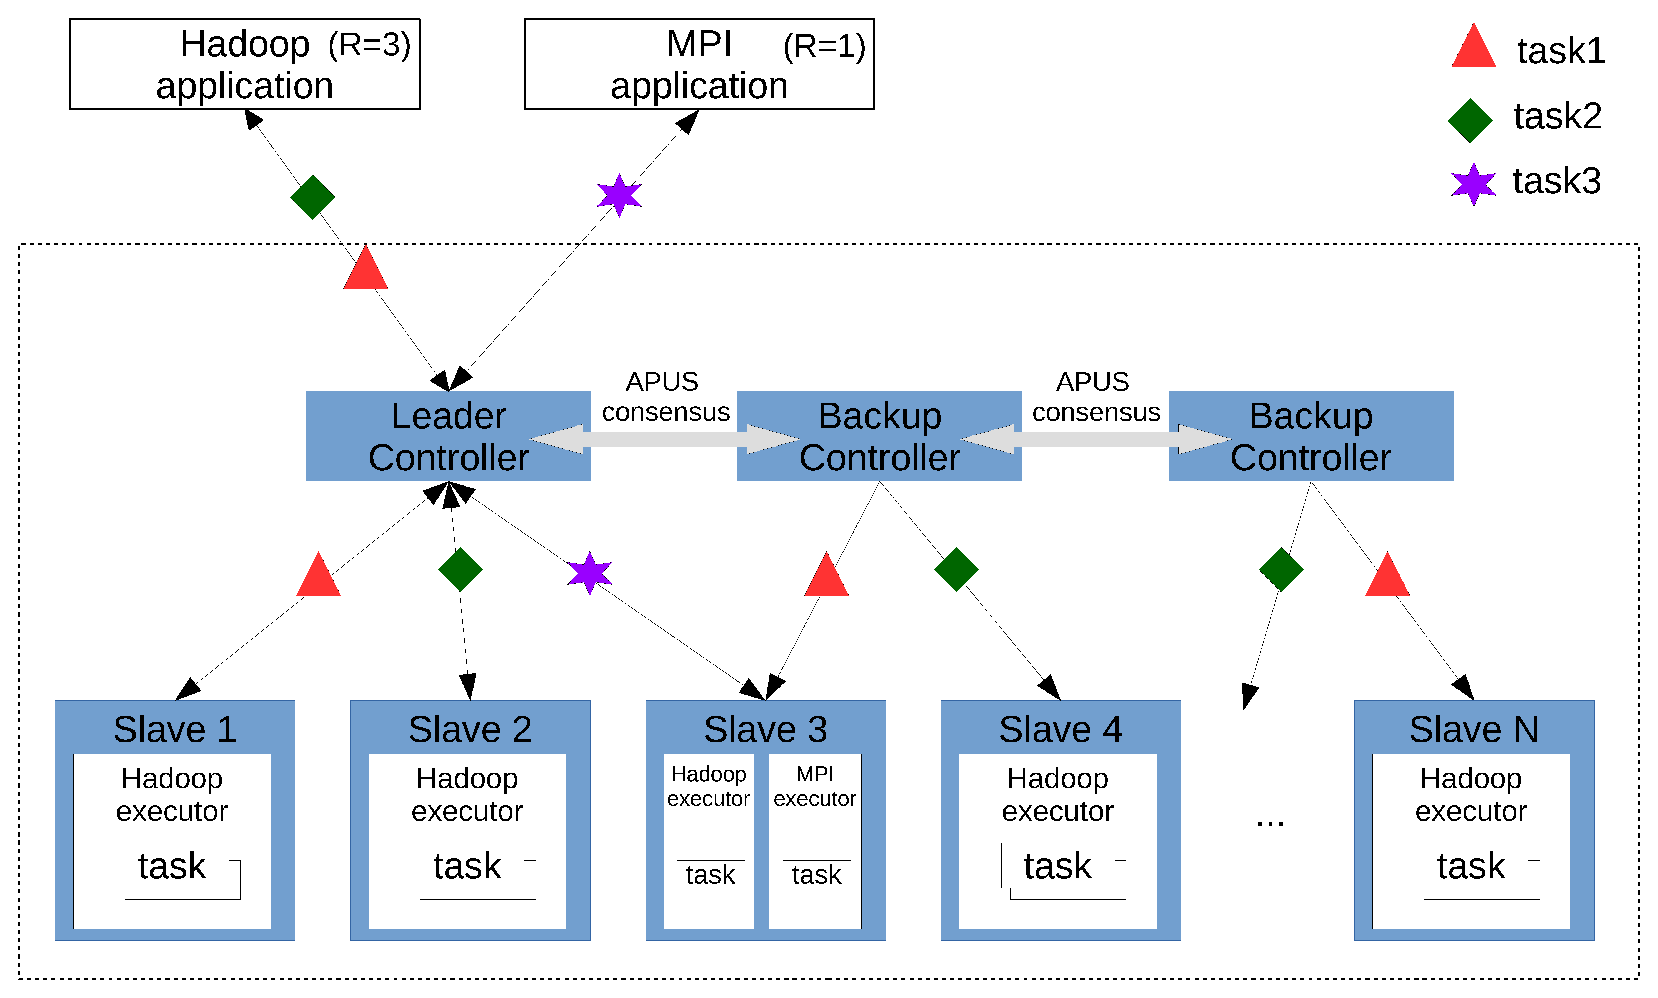
\includegraphics[width=0.34\textheight]{figures/scheduler_arch.eps}
        \vspace{-.25in}
        \caption{The \tripod fault-tolerant scheduler.}
        \label{fig:scheduler-arch}
    \end{minipage}
    \begin{minipage}{0.51\textwidth}
        \vspace{-.2in}
        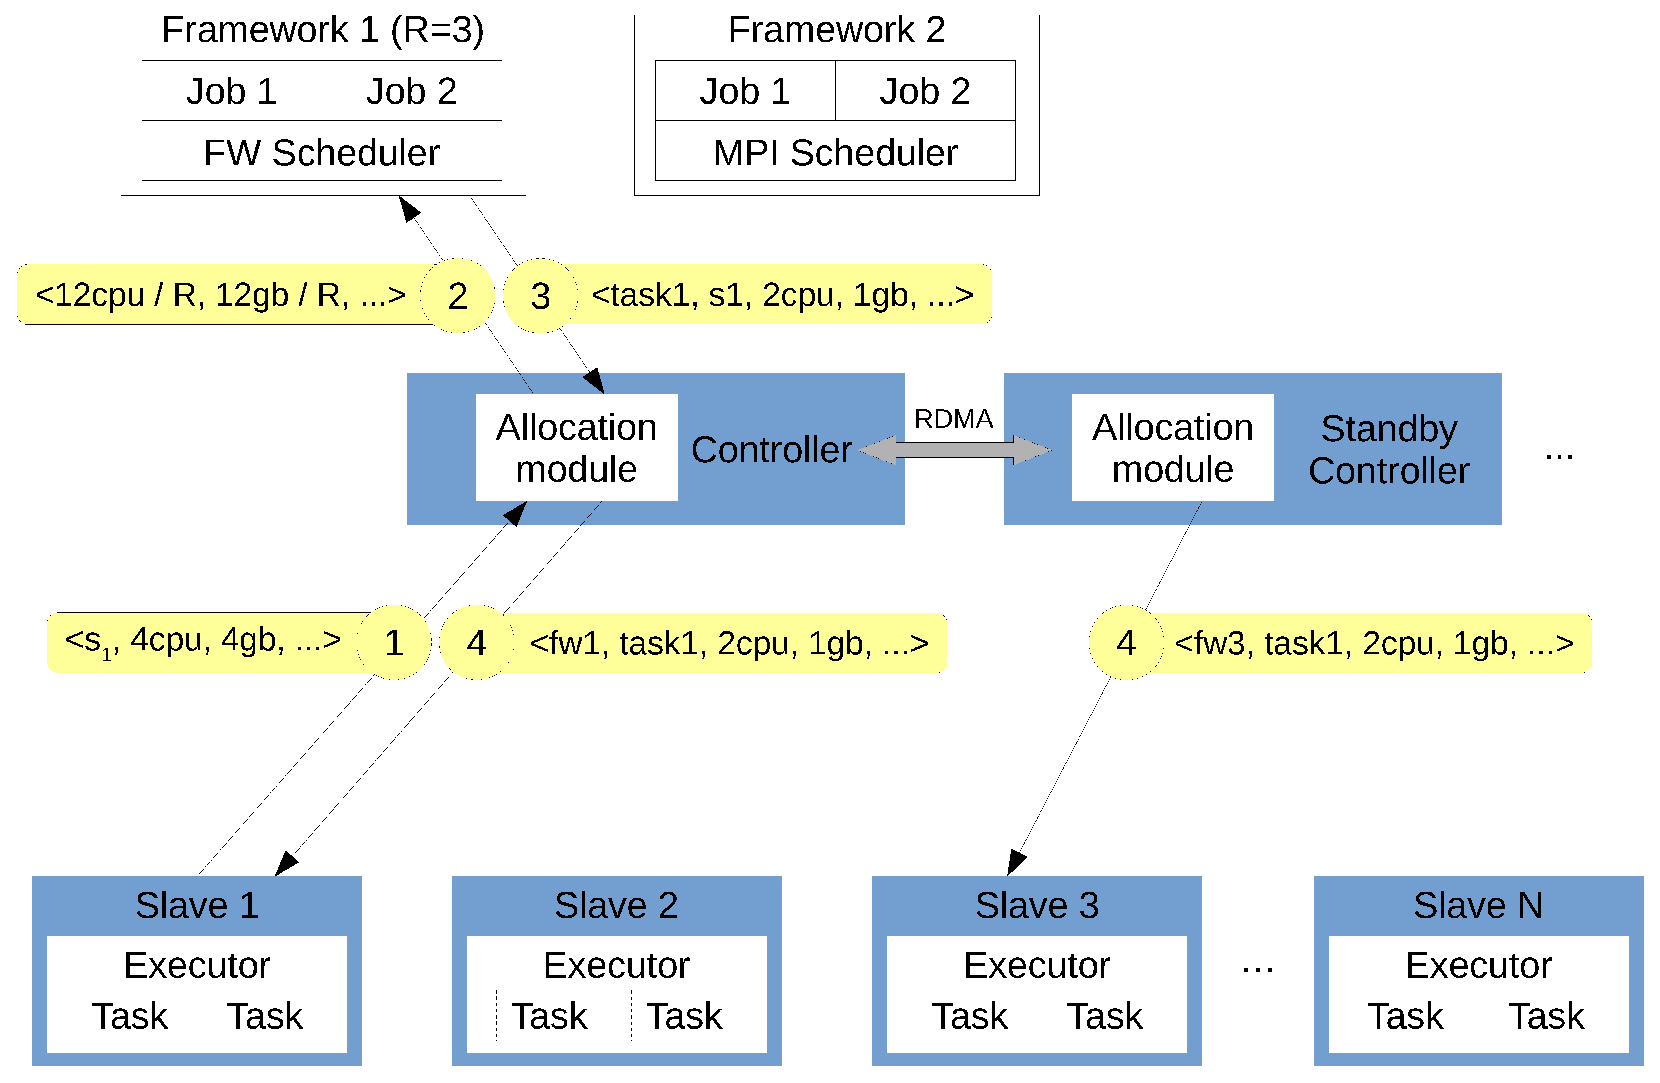
\includegraphics[width=0.34\textheight]{figures/scheduler_flow.eps}
        \vspace{-.05in}
        \caption{The replication-aware resource allocation scheme.}
        \label{fig:scheduler-workflow}
    \end{minipage}
\end{figure}

\vspace{-.15in}\subsubsection{Replication-aware resource allocation scheme}
\label{sec:workflow}\vspace{-.075in}

Figure~\ref{fig:scheduler-workflow} shows \tripod's scheme on scheduling jobs 
with four steps. This scheme is similar to that in Mesos except the second 
and fourth steps. These two steps \tripod abstract away the replication logic 
in its resource offers and allocations from the application. An application runs 
as if \xxx does not replicate any of its jobs, and \tripod transparently 
handles all the replication logic.

In the first step, slave machines periodically report their available computing 
resources (\eg, CPU cores and memory) to the leader controller. In the second 
step, instead of offering the available resources aggregated from slave 
machines, \tripod divides the amount of resources by each application's \vv{R} 
value and then sends a resource offer to the application. The goal is to 
reserve enough resources for \tripod to replicate a job with \vv{R} copies.

In the third step, an application scheduler submits jobs to the leader 
controller. The leader controller then invokes a consensus on this job by 
carrying the resource offer made to the application.

Once a majority of controllers agrees on executing this job, each controller 
does the fourth step. It schedules this job on an available slave machine 
according to the resource offer. To prevent controllers putting the same job on 
the same slave machine, the leader controller first makes an assignment on 
which controller should run this job on which slave machine, it then carries 
this assignment in its consensus request. Once a consensus on this job is 
reached, each controller follows this assignment.

% Two figures: one is TRIPOD arch. The other is TRIPOD results from the workshop 
% paper. Figure~\ref{fig:scheduler-arch} and Figure~\ref{fig:scheduler-workflow} 
% and Figure~\ref{fig:scheduler-latency}.


\para{Availability v.s. resource consumption.} \tripod is designed to make a
mission-critical application highly available by leveraging \vv{R} times of 
resources than the application's native, unreplicated execution. We deemed this 
extra resource consumption reasonable, because a major trend is that an 
application runs on more and more computers, thus minor computer failures tend 
to happen more likely. Such failures may turn down the entire application and 
cause if the failure computer runs a critical computation. For instance, Both 
NYSE and Nasdaq have experienced 
outage of their whole site~\cite{nyse:halt} or specific IPO 
events~\cite{facebook:ipo:delay} due to minor machine errors. 
In addition, social-networking applications like Facebook has 
strong fault-tolerance requirements, because minor machine failures have turned 
down the whole Facebook site for several times in the last few 
years~\cite{facebook:outage}, costing huge money lost. 
% for two reasons.
% Second, it is already a common practice to replicate critical computations by 
% using \vv{R} times of resources, and doing so can improve both availability and 
% performance. For instance, Scatter~\cite{scatter:sosp11} runs 8$\sim$12 
% replicas in a \paxos group to order client requests, and it lets replicas reply 
% requests in parallel. A bigger group size will improve Scatter throughput. 
% Moreover, several recent replication 
% systems~\cite{eve:osdi12,rex:eurosys14,crane:sosp15} 
% improve the availability of general server applications (\eg, 
% \mysql~\cite{mysql}) by replicating them.

% Therefore, \tripod's design favors more on availability and performance 
% (low consensus latency). It's design tends to use \vv{R} times of resources 
% compared to traditional applications. We argue that this extra resource 
% utilizations are acceptable for critical applications, because if they have 
% high 
% demand on availability and response times, they can often tolerate costs on 
% computing resources (\eg, trading and medical platforms).



\para{Preliminary results.} We built and published a \tripod prototype 
in~\cite{tripod:apsys16}. To evaluate a typical social-networking application, 
we ran \tripod with \memcached~\cite{memcached}, a popular key-value store used 
by Twitter and financial platforms~\cite{nosql:finance}. Compared to 
\memcached's unreplicated execution, \tripod incurred merely a \tputoverhead 
overhead in throughput and \latencyoverhead in response time.
% This protocol was 40.1X faster than \zookeeper, a traditional replication
% protocol~\cite{calvin:sigmod12} which runs on TCP/IP.

% Disable the figure for now. Not much information.
% \begin{figure}[!htb]
% \centering
% 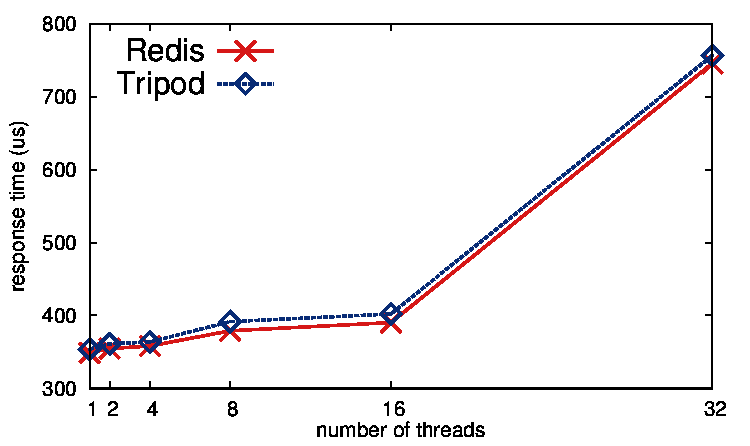
\includegraphics[width=0.34\textheight]{figures/scheduler_latency.ps}
%         \vspace{0.1in}
%         \caption{Performance overhead of scheduler.}
%         \label{fig:scheduler-latency}
% \end{figure}

\para{Future work.} Our \tripod development will go along two directions. 
First, currently our replication and resource allocation scheme is tied with 
\mesos. We will study other popular schedulers and summarize their 
resource allocation scheme patterns, and we will develop a general, 
scheduler-agnostic scheme. Second, we will study new differential replication 
schemes, so that we can flexibly assign different \vv{R} values to different 
components of an application, getting both satisfiable availability and optimal 
resource consumption.

\vspace{-.15in}\subsection{Objective 3: building a fault-tolerant VM to improve 
application availability}\label{sec:vm}\vspace{-.075in}

%% TBD: must emphasis that primary-backup or migration will clean up dirty 
% % pages after the transfer, otherwise the tree will become bigger and bigger 
% and we have not optimization.

Virtual machines (VM) infrastructures (\eg, Amazon EC2~\cite{amazon:vpc} and 
OpenStack~\cite{openstack}) are widely deployed in datacenters and clouds 
because they can provide a virtualized abstraction of computing resources to 
different applications and enforce strong utilization isolation and security. 

As mentioned in related work (\S\ref{sec:others-work}), primary-backup and live 
migration are two common techniques for improving VM fault-tolerance and 
resource utilization. They both are invoked frequently when serving requests or 
the resources on local VM are tight. They both move all memory pages modified 
by applications (\ie, dirty pages) from a local VM to a remote one, so they 
both have the problems of significant application downtime (\eg, 8 seconds in a 
live migration system vMotion~\cite{vmotion:atc05}) and network bandwidth.

A key reason that causes these problems is that these approaches have only one 
actual application execution on one VM. Therefore, when dirty pages are 
transfered to a remote computer, substantial time and network bandwidth are 
consumed.




% Therefore
% Mainly introduce EC2, Openstak. VM only.

% Briefly introduce VM fault-tolerance techniques. Primary-backup. Remus. 
% Hypervisor replication (old paper). FaRM.
% 
% Talk about migration. It is similar to primary-backup, but mainly for load 
% balance, not to overcome failures. Main approach is live migration that aims to 
% reduce application down time. VMotion.

% However, there is still substantial down time and resource consumption. E.g., 
% vMotion, for memory intensive applications, the down time can be up to 30 
% seconds. As migration tends to invoke frequently for load balancing, 
% consolidation, energy saving, this downtime may incur big money lost for cloud 
% deployers.

% When doing migration, both the local computer and the migration destination 
% computer incur big resource consumption. This is contraditive to the motivation 
% of migration: reduing computer loads on the local computer.

\vspace{-.15in}\subsubsection{Integraging \falcon with VM} 
\label{sec:vm-arch}\vspace{-.075in}

% \begin{figure}[!htb]
% \centering
% \vspace{-.2in}
% 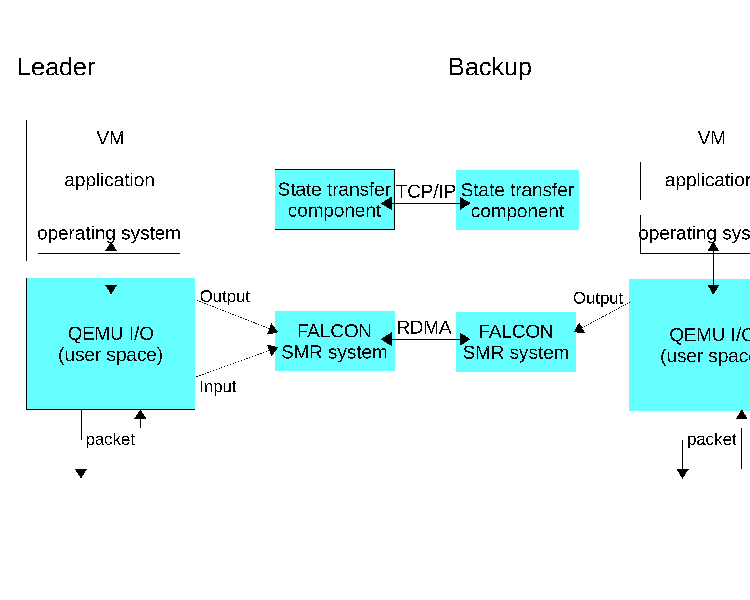
\includegraphics[width=0.25\textheight]{figures/vm_arch.ps}
%         \vspace{-.3in}
%         \caption{The \falcon and KVM eco-system.}
%         \label{fig:vm-arch}
%         \vspace{-.2in}
% \end{figure}

\begin{figure}[!htb]
%     \begin{minipage}{.49\textwidth}
%         \vspace{-.2in}
%         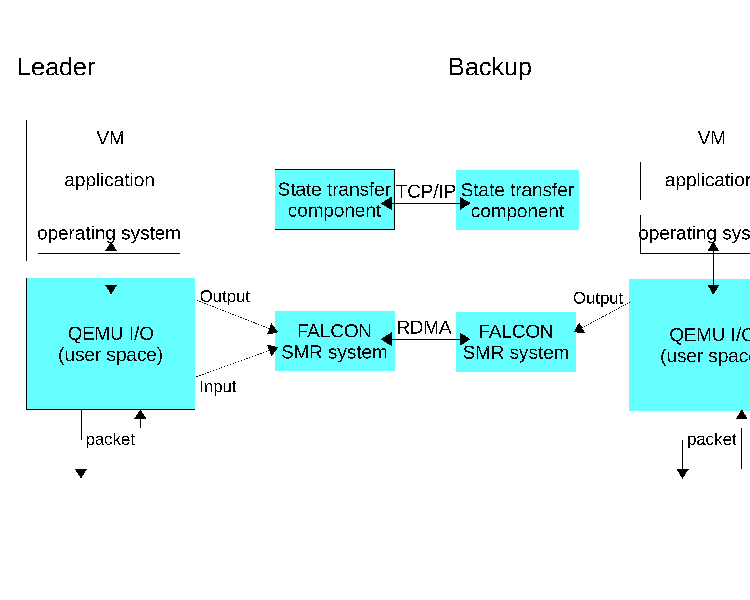
\includegraphics[width=0.34\textheight]{figures/vm_arch.ps}
%         \vspace{-.3in}
%         \caption{A new fault-tolerant VM for improving application 
% availability.}
%         \label{fig:vm-arch}
%     \end{minipage}
    \begin{minipage}{0.47\textwidth}
        \vspace{-.15in}
        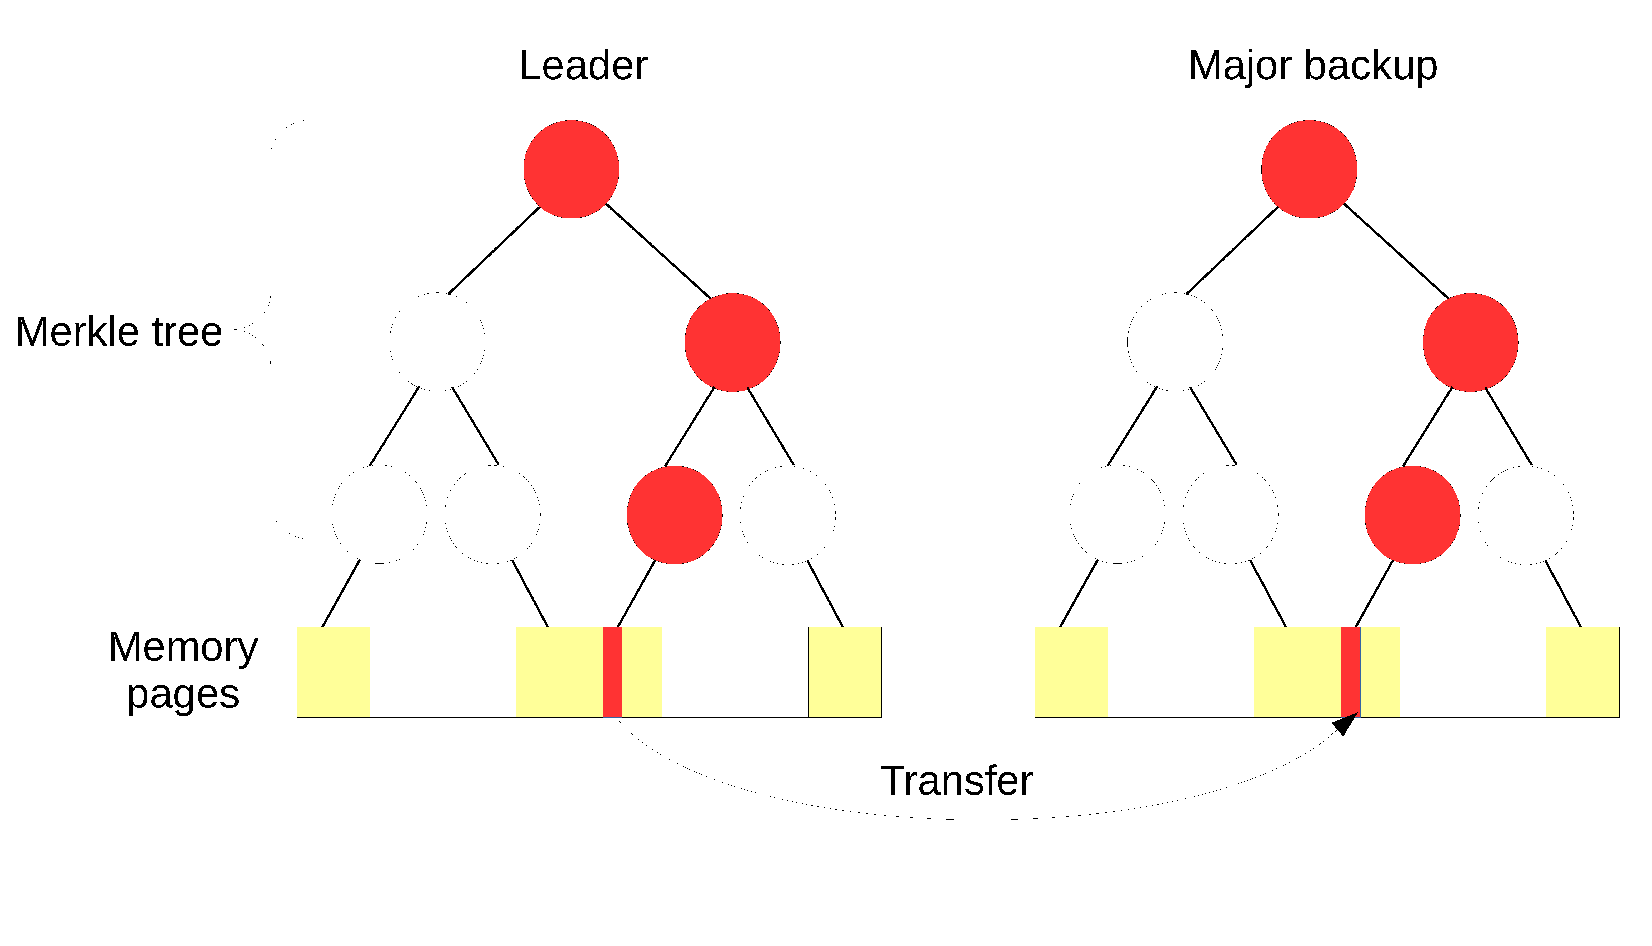
\includegraphics[width=0.34\textheight]{figures/tree.ps}
        \vspace{-.4in}
        \caption{Data structures on tracking different memory pages 
across VMs. Diverged pages and their parent nodes are marked red by 
\textbf{Algorithm 1}.}
        \label{fig:vm-tree}
    \end{minipage}
    \begin{minipage}{0.52\textwidth}
      \vspace{-.1in}
      \centering
      \begin{algorithm}[H]
      \DontPrintSemicolon
      \scriptsize
      \SetCommentSty{textrm}
      \SetKwInOut{Input}{Input}
      \SetKwInOut{Output}{Output}
      \Input{The root of merkle tree on leader, $root$}
      \Output{Different memory pages between leader and replica, $pages$}
      
      \SetKwBlock{Titlea}{Track($root$)}{end}
      \Titlea {
        $diverged$ $\leftarrow$ empty sequence \;
        $pages$ $\leftarrow$ empty sequence \;
        $diverged$ $\leftarrow$ \textbf{FALCON}(root, root.left(), 
root.right()) \;
        \For {{\rm $i$ $\leftarrow$ $diverged$.push\_front()}} {
          \If {{\rm $i$ is\_leaf()}} {
            $pages$.append($i$) \;
          }
          \Else {
            $diverged$.append(\textbf{FALCON}($i$, $i$.left(), 
$i$.right()) \;
          }
        }
        \Return $pages$ \;
      }
      \caption{Tracking different memory pages}
      \label{alg:slice}
      \end{algorithm}
    \vspace{-.1in}
    %     \caption{Sketch of path slicing algorithm}

%         \label{fig:algo}

\end{minipage}
\end{figure}




Fortunately, \paxos-based replication can construct multiple equivalent 
executions on multiple computers due to its reliability and consistency 
guarantee. To ensure high application availability, we can just run \paxos 
make VM replicas process same sequence of inputs, then most dirty memory 
pages across replicas are the same and they need not be transfered.

We propose a new fault-tolerant VM by integrating \falcon into the hypervisor 
layer of popular VMs. Specifically, we choose the popular KVM~\cite{kvm} for 
three main reasons. First, KVM is an open source hypervisor carried in Linux. 
Second, it provides \vv{tap\_send()}, an input capturing API at its hypervisor 
layer. This API allows \falcon to intercept network inputs of the leader VM and 
transparently replicates same inputs on backup VMs. Third, this KVM API runs in 
userspace, which allows \falcon's RDMA to work (all current commodity RDMA 
features run in userspace).

%% Consume same resources as primary-backup.
We carefully design our VM to achieve same level of resource consumption as 
existing VM fault-tolerance techniques. An existing primary-backup technique 
consumes $2\times\vv{R}$ resources compared to unreplicated executions as it 
maintains a primary execution and a backup execution. Although typical 
\paxos-based replications consume $3\times\vv{R}$ resources, our VM design 
mitigates this consumption by assigning one backup as the \emph{major backup} 
which agrees on and executes input requests, and the other backup the 
\emph{standby backup} which only agrees on requests without executing them. The 
major backup then periodically (one minute, by default) does checkpoints on 
application states and propagate the checkpoints to the standby backup. Such a 
checkpoint does not perturb the leader to process requests because the leader 
and standby backup still form a majority and agree on requests rapidly. Once the 
leader fails, \falcon gives the major backup a high priority to become the new 
leader.

This design has three important benefits: (1) our new VM fault-tolerance 
technique consumes roughly same $2\times\vv{R}$ computing resources as existing 
techniques; (2) a \paxos majority group still holds; (3) this design is pratical 
because even if the standby backup is elected as the new leader, it can extract 
checkpoints and catch up with the old leader quickly.

% Figure~\ref{fig:vm-arch} shows the architecture of the eco-system. To provide 
% the same fault-tolerance guarantee with primary-backup, a typical replication 
% factor of this eco-system is \vv{R=3}. 

% A key benefit of such a \paxos-based VM replication over primary-backup is that 
% its leadership is strongly consistent (through a majority agreement, which 
% primary-backup lacks), and it saves the bandwidth consumption for transferring 
% application execution states in primary-backup.

\vspace{-.15in}\subsubsection{Tracking minor diverged dirty pages across VM 
replicas}
\label{sec:tracking}\vspace{-.075in}

By enforcing same inputs across VM replicas, most dirty pages due to serving 
inputs are already made the same, but some minor pages may still diverge across 
replicas (\eg, due to data races~\cite{lu:concurrency-bugs}). Our new VM 
efficiently track and transfer diverged pages across VM replicas with two novel 
parts: (1) proposing an efficient \vv{log(N)} algorithm to track diverged pages, 
and (2) leveraging \falcon protocol to perform efficiently and reliably 
transfer diverged pages across replicas. A common data structure to track dirty 
pages is a Merkle tree~\cite{eve:osdi12} on each replica. As shown 
in Figure~\ref{fig:vm-tree}, once a physical page is modified, our VM 
hypervisor handler appends this page as a leaf to this Merkle () and recomputes 
a hash based on the page content for its parents. Such a data tree is efficient 
because if the root hashes of two trees are the same, then all dirty pages 
(all leaves) are the same.

% Three steps.
Our new VM design poses a new interesting challenges to this Merkle tree. 
Unlike previous works that three leaves are static~\cite{eve:osdi12} 
(\ie, they statically treat global variables in application code as leaves), 
the leaves in our trees are dynamic as they are dirty pages. As the dirty pages 
across replicas can be different, the structures (\ie, the number of internal 
nodes) of Merkle trees across replicas can be different and thus comparing roots 
makes no sense.

Our new VM address this challenge by introducing a tree adjustment phase. Our 
technique works with four steps. First, after serving a request, the leader 
sends a dirty page bitmap provided by KVM to the standby backup. The backup 
takes its own bitmap, does a union on the two bitmaps and sends back to leader. 
Second, both leader and the standby backup do a tree adjustment with the union 
bitmap (\eg, even if a page is not dirty on the leader, it is append to the 
leader's tree), so that leader and the backup's trees have same structure. 
Second, the leader invokes \textbf{Algorithm 1} to track the diverged pages 
(leaves) across replicas and mark them red. Third, leader transfer the diverged 
pages to the standby backup. Fourth, both leader and the standby mark all dirty 
pages as clean and clear their threes.

The efficacy of our algorithm depends on a key insight: the diverged dirty 
pages between the leader and backups are rare. To verify this insight, we ran 
three real-world appliations, MySQL~\cite{mysql}, MongoDB~\cite{mongodb}, and 
Memcached~\cite{memcached}, on two KVMs and provide same real-world request 
workloads~\cite{sysbench} on the two VMs. For these three applications, we 
found that 2.4GB to 7.3GB memory pages were dirty after serving requests. 
Existing primary-backup or migration techniques need to transfer all dirty 
pages from primary to backup. We also found that only 16.4MB to 107.8MB of 
these dirty pages were different between two VMs. This preliminary study implies 
that our proposed algorithm can save up to 99.8\% of transfered pages 
compared to existing techniques, saving most time and network bandwidth.

% To do this, each replica 
% maintains a Merkle tree kept 
% updating from the dirty pages. By "dirty", we mean the memory page has been 
% modified since last synchronization. One problem here is that each VM may have 
% dirtied different pages. This leads to different structures of Merkle trees and 
% they are not comparable. \xxx addresses this problem using a fast method as 
% follows:

% \begin{small} \textit{(We use $A$ to denote the diverged replica; it will fetch 
% state 
% from replica $B$)} \end{small}
% \begin{enumerate}
% \item $A$ sends its dirty page bitmap $M_A$ to $B$.
% \item $B$ does a \textit{bitwise or} calculation \ $M_{union} = M_A | M_B $, 
% and sends $M_{union}$ back to $A$.
% \item $A$ and $B$ both update their own Merkle tree according to $M_{union}$. 
% $A$ sends its updated Merkle tree to $B$. 
% \item $B$ does a comparison on both Merkle tress to find the differences, as 
% illustrated in Figure~\ref{fig:tree}.
% \end{enumerate}

% Our method is efficient for two reasons. First, it only transfers the different 
% pages between replicas. Because we have made consensus on inputs and we can 
% turn off \textit{Address Space Layout Randomization} to trade for correctness, 
% the difference rate will be really small. Second, the use of Merkle tree 
% optimizes the time complexity of comparison between memory states to $O(\log 
% n)$.

% Describe the infrastructure. Take Ning's figure. Hypervisor. tap\_send().

% \vspace{-.15in}\subsubsection{\paxos-based Live Migration} 
% \label{sec:vm-migration}\vspace{-.075in}
% 
% Interestingly, this replication ability not only provides high 
% availability for fault-tolerance (suitable for the primary-backup scenario), 
% but can also greatly save resource consumption if fault-tolerance is not a 
% major concern (suitable for the live migration scenario). Consider the live 
% migration scenario, \paxos backups can only agree on inputs without actually 
% executing them, then the overall application execution consumes almost same 
% resources as the unreplicated one. A backup now can just absorb occasional, 
% periodical application checkpoints from the leader when the leader replica is 
% idle, and catches up with the leader when a migration destination is decided on 
% this backup.
% 
% % We propose our own replication approach. The non-leader only agree on new 
% % inputs, they can opt to execute requests or absorb periodic checkpoints.
% Leveraging this idea, we propose a fast, network bandwidth-friendly live 
% migration approach called ``\paxos-based live migration". A key benefit of this 
% approach is that, now migration does not require transferring all execution 
% states of application, but only transferring the \paxos leadership (almost as 
% fast as \paxos consensus latency) to a destination backup which has idle 
% resources. To increase the chance on finding a proper destination, we can 
% leverage \falcon's high availability to run many backups within a datacenter.

% This approach is othorgnal to the VM replication. 
% This \paxos-based live migration approach contains four steps. First, in 
% normal case, the current computing instance (the leader) just agrees on 
% incoming inputs with backups using \falcon. A set of backups run on highly 
% loaded computers and agree on inputs (also record the inputs persistently). 
% 
% Second, the leader does a periodical checkpoint when it's idle (no incoming 
% requests), and sends the checkpoint to the backups. The backups only keeps 
% the latest checkpoint and discards prior ones.
% 
% Third, when the VM invokes a migration on the leader computer, it uses a 
% standard migration mechanism to determine which backup should be the migration 
% destination (the next leader). Then, the destination extracts the latest
% checkpoint on local computer, restores the application state, and then catches 
% up with the leader with executing the recorded but not executed inputs.
% 
% Fourth, we invoke a \falcon protocol level operation: migration the 
% leadership, which is similar to a traditional \paxos leader election 
% process~\cite{paxos:practical}, but we just explicitly decide the destination 
% computer as the new leader. \falcon's protocol handles various failure 
% scenarios (\eg, the destination computer crashes during the migration) as its 
% \paxos nature.

% TBD: mention the leader election latency in Objective 2.
% Analysis: this approach incurs almost zero time and resource for a few reasons. 
% First, the leadership migration is fast (tens of micro seconds). Second, no 
% frequent execution state transfer during the migration time, only at the 
% leader's idle time. Third, robust to various scenarios (\eg, destination fails 
% during the migration), thanking to \paxos.

\para{Future work}. We plan to fully implement our new fault-tolerant VM, 
including integrating \falcon with popular VMs and developing our novel 
efficient memory tracking algorithm. We will compare the performance overhead 
of our implementation with existing VM primary-backup techniques (\eg, 
Remus~\cite{remus:nsdi08}) and quantify the saving on transfered pages. We will 
also broadly apply our technique to build a fast, lightweight VM live migration 
technique for improving resource utilization and saving datacenter 
energy~\cite{vmotion:atc05}.


% % TBD: need a new replication approach name.
% \vspace{-.15in}\subsubsection{Idea I: Hybrid Replication} 
% \label{sec:defense-arch}\vspace{-.075in}
% 
% TBD.

\vspace{-.15in}\subsection{Research Plan} \label{sec:plan}\vspace{-.075in}

This project will require two PhD students S1 and S2 to work for 
three years. In the first year, S1 will design and fully implement the \falcon 
protocol (part of \textbf{Objective~1}), and S2 will evaluate its performance 
and robustness on various real-world storage applications (part of 
\textbf{Objective~2}). In the second year, S1 will 
integrate \falcon to a scheduler \mesos (part of \textbf{Objective~2}), and S2 
will make \falcon and KVM form an eco-system (part of \textbf{Objective~3}). In 
the third year, S1 and S2 will respectively study the efficacy of their systems 
built Object 2 and Object 3 with real-world applications, including big data 
applications.
% Both students will 
% involve theoretical methods, implement real software systems, and 
% perform real-world study.
% The PI will supervise the students by providing 
% advice concerning both theoretical and systems implementation levels.


